\documentclass[12pt]{article}
\usepackage{xeCJK}
\usepackage{amssymb,tikz,pdftexcmds,xparse}
\usepackage{url}
\usepackage{titlesec}

\usepackage{indentfirst}

% Adjust spacing for section
\titlespacing*{\section}
{0pt} % Left spacing
{10pt} % Spacing before the section
{4pt}  % Spacing after the section

% Adjust spacing for subsection
\titlespacing*{\subsection}
{0pt} % Left spacing
{8pt} % Spacing before the subsection
{3pt}  % Spacing after the subsection

% Adjust spacing for subsubsection
\titlespacing*{\subsubsection}
{0pt} % Left spacing
{12pt} % Spacing before the subsubsection
{1pt}  % Spacing after the subsubsection


\tikzset{box/.style={
    minimum size=0.225cm,
    inner sep=0pt,
    draw,
  },  
  insert mark/.style={
    append after command={%
         node[inner sep=0pt,#1]
           at (\tikzlastnode.center){$\checkmark$}
     }     
  },
  insert bad mark/.style={
    append after command={%
         [shorten <=\pgflinewidth,shorten >=\pgflinewidth]
         (\tikzlastnode.north west)edge[#1](\tikzlastnode.south east)
         (\tikzlastnode.south west)edge[#1](\tikzlastnode.north east)
     }     
  },
}

\makeatletter
\NewDocumentCommand{\tikzcheckmark}{O{} m}{%
  \ifnum\pdf@strcmp{#2}{mark}=\z@%
    \tikz[baseline=-0.5ex]\node[box,insert mark={#1},#1]{};%
  \fi%
  \ifnum\pdf@strcmp{#2}{bad mark}=\z@%
    \tikz[baseline=-0.5ex]\node[box,insert bad mark={#1},#1]{};%
  \fi%
  \ifnum\pdf@strcmp{#2}{no mark}=\z@%
    \tikz[baseline=-0.5ex]\node[box,#1]{};%
  \fi%
}
\makeatother


% Redefining maketitle
\makeatletter
\renewcommand{\maketitle}{
  % \begin{center}
    {\LARGE \@title \par}      % Title in large font
    % \vspace{2mm}               % Space between title and author
    % {\large \@subtitle \par}      % Subtitle in large (but smaller than title) font
    % \vspace{2mm}               % Space between title and author
    {\large \@author \par}     % Author in large (but smaller than title) font
    % Date is removed, so no command for date here
  % \end{center}
  % \vspace{5mm}                 % Space after the title block
}
\makeatother

% Language setting
% Replace `english' with e.g. `spanish' to change the document language
\usepackage[english]{babel}

% Set page size and margins
% Replace `letterpaper' with `a4paper' for UK/EU standard size
\usepackage[letterpaper,top=2cm,bottom=2cm,left=2cm,right=2cm,marginparwidth=1.75cm]{geometry}

% Useful packages
\usepackage{amsmath}
\usepackage{graphicx}
\usepackage[colorlinks=true, allcolors=blue]{hyperref}
\usepackage{listings}
\usepackage{color}
\usepackage{minted}

% https://www.overleaf.com/learn/latex/Positioning_images_and_tables#Basic_positioning
% To position the image to the centre
\usepackage[export]{adjustbox}  

\usepackage{xcolor}
\usepackage{xparse}
\usepackage{blindtext}
\usepackage{hyperref}   % For hyperlinks

\usemintedstyle{manni}

\NewDocumentCommand{\codeword}{v}{%
% \texttt{\textcolor{blue}{#1}}%
\texttt{\textcolor{black}{#1}}%
% \mint{html}|v|%
}

% \lstset{language=C,keywordstyle={\bfseries \color{blue}}}

\definecolor{dkgreen}{rgb}{0,0.6,0}
\definecolor{gray}{rgb}{0.5,0.5,0.5}
\definecolor{mauve}{rgb}{0.58,0,0.82}

\lstset{frame=tb,
  % language=Java,
  language=Python,
  aboveskip=3mm,
  belowskip=3mm,
  showstringspaces=false,
  columns=flexible,
  basicstyle={\small\ttfamily},
  numbers=none,
  numberstyle=\tiny\color{gray},
  keywordstyle=\color{blue},
  commentstyle=\color{dkgreen},
  stringstyle=\color{mauve},
  breaklines=true,
  breakatwhitespace=true,
  tabsize=2
}

\title{MTH786P Project - Diabetes Prediction}
\author{Thanh Trung Vu - 230849442}

\usepackage[utf8]{inputenc}
\usepackage[english]{babel}
\usepackage{biblatex}
\addbibresource{references.bib}

\begin{document}

\setlength\parskip{0.5em plus 0.1em minus 0.2em}

% \vspace{-30pt}


% \begin{figure}
%     \centering
%     
\includegraphics[width=0.3\linewidth]{images/QMUL logo.png}
%     % \caption{Enter Caption}
%     % \label{fig:enter-label}
% \end{figure}

% \vspace{-30pt}

% \maketitle

% {\large \textbf{MTH786P Machine Learning with Python, Semester A, 2023/24}}

% {\large \textbf{Final project}}

{\large \textbf{MTH786P Final Project - Diabetes Prediction}}

{\large \textbf{Thanh Trung Vu - 230849442}}

% \vspace{-12pt}

\section{Introduction}

% \subsection{Overview}

\indent This project utilises the Diabetes Dataset\cite{kaggle-diabetes}, originally sourced from the National Institute of Diabetes and Digestive and Kidney Diseases. The primary goal is to develop a predictive model that accurately determines the presence of diabetes in patients based on various diagnostic measurements.

The project begins with a comprehensive examination of the dataset, involving an analysis
of each feature, followed by appropriate data processing. Subsequently, different classification
algorithms, namely K-Nearest Neighbors (KNN), Logistic Regression, and Support Vector Machine
(SVM), are discussed and implemented. The models are then trained and evaluated using specified
performance metrics, including accuracy and F1 score. In the final stage, the results are analysed
to compare the effectiveness of the different models and interpreted to see which features hold the highest
predictive power in addressing the diabetes prediction problem.



\section{Data Analysis and Processing}



\subsection{Preliminary Analysis}

\indent The dataset consists of diagnostic data from 768 female individuals of Pima Indian heritage, all aged 21 or above. It includes the following eight features and one target variable. All data are numerical with no missing values (NaN).

\vspace{-9pt}

\begin{itemize}
\setlength\itemsep{-0.3em}
\item $\mathtt{Pregnancies}$: Number of times pregnant.
\item $\mathtt{Glucose}$: Plasma glucose concentration post 2 hours in an oral glucose tolerance test.
\item $\mathtt{BloodPressure}$: Diastolic blood pressure (mm Hg).
\item $\mathtt{SkinThickness}$: Triceps skin fold thickness (mm).
\item $\mathtt{Insulin}$: 2-hour serum insulin (mu U/ml).
\item $\mathtt{BMI}$: Body mass index, calculated as weight in kilograms divided by the square of height in meters (kg/m$^2$).
\item $\mathtt{DiabetesPedigreeFunction} \quad \mathtt{(DPF)}$: A function indicating diabetes pedigree.
\item $\mathtt{Age}$: Age in years.
\item $\mathtt{Outcome}$: Binary variable indicating diabetes diagnosis (0 = No, 1 = Yes).
\end{itemize}

\vspace{-3pt}

We can see that this dataset contains information that could be valuable in predicting diabetes.
It seems plausible that there is a significant link
between diabetes and variables such as glucose concentration and insulin levels. 
Additional indicators, such as age and body mass index (BMI), may also provide insights into an individual's overall health, which might aid in forecasting diabetes risk.
One could, for instance, speculate that a person with a high BMI is at higher risk of obesity, which in turn may increase their chances of developing diabetes.


Upon further analysis, an initial assessment reveals certain anomalies in features such as $\mathtt{Glucose}$, $\mathtt{BloodPressure}$, $\mathtt{SkinThickness}$, $\mathtt{Insulin}$, and $\mathtt{BMI}$. The presence of biologically implausible zero values in these features suggests missing or incorrect data. Since the number of features is reasonably low, a closer examination of each feature is carried out which can help us decide the appropriate data cleaning strategies.


\subsection{Feature-Specific Analysis}

\begin{table}[h]
\begin{center}
    
\begin{tabular}{lrrrrrrrr}
\hline
               & count & mean  & std   & min  & 25\%  & 50\%  & 75\%  & max   \\ \hline
$\mathtt{Pregnancies}$    & 768.0 & 3.85  & 3.37  & 0.00 & 1.00  & 3.00  & 6.00  & 17.00 \\
$\mathtt{Glucose}$        & 768.0 & 120.89& 31.97 & 0.00 & 99.00 & 117.00& 140.25& 199.00\\
% BloodPressure  & 768.0 & 69.11 & 19.36 & 0.00 & 62.00 & 72.00 & 80.00 & 122.00\\
% SkinThickness  & 768.0 & 20.54 & 15.95 & 0.00 & 0.00  & 23.00 & 32.00 & 99.00 \\
% Insulin        & 768.0 & 79.80 & 115.24& 0.00 & 0.00  & 30.50 & 127.25& 846.00\\
% BMI            & 768.0 & 31.99 & 7.88  & 0.00 & 27.30 & 32.00 & 36.60 & 67.10 \\
% DPF            & 768.0 & 0.47  & 0.33  & 0.08 & 0.24  & 0.37  & 0.63  & 2.42  \\
% Age            & 768.0 & 33.24 & 11.76 & 21.00& 24.00 & 29.00 & 41.00 & 81.00 \\
% Outcome        & 768.0 & 0.35  & 0.48  & 0.00 & 0.00  & 0.00  & 1.00  & 1.00  \\ \hline
\end{tabular}

% \caption{Key statistics of the features $\mathtt{Pregnancies}$ and $\mathtt{Glucose}$}
\vspace{6pt}


Key statistics of the features $\mathtt{Pregnancies}$ and $\mathtt{Glucose}$


\end{center}

\end{table}

In this section, we demonstrate the analysis and processing of two features: \texttt{Pregnancies} and \texttt{Glucose}. The analysis and processing of the remaining features follow a similar methodology.


Regarding the feature $\mathtt{Pregnancies}$, we can see that the number of pregnancies ranges from 0 to 17. With an average of approximately 3.8 pregnancies per individual, the data exhibits a reasonable range, given the demographic profile of the participants. 
Large values such as 17 and 15 may raise concerns, but we can disregard them for the time being.



\begin{center}
    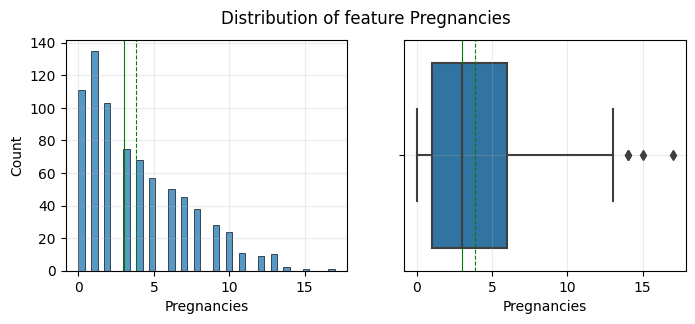
\includegraphics[width=0.7\linewidth]{images/dist - pregnancies.png}
    
    \vspace{-8pt}
    
    % \caption{Distribution of the feature $\mathtt{Pregnancies}$}
    \label{fig:dist-pregnancies}
\end{center}

\vspace{-6pt}

The feature $\mathtt{Glucose}$ also contains zero values. However, glucose measurements of zero are biologically implausible and likely indicate missing data.

\vspace{-6pt}

\begin{center}
    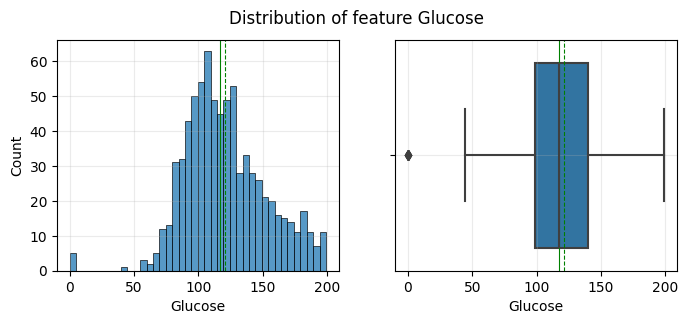
\includegraphics[width=0.7\linewidth]{images/dist - glucose.png}
    
    \vspace{-8pt}
    
    % \caption{Distribution of the feature $\mathtt{Glucose}$}
    \label{fig:dist-glucose}
\end{center}

\vspace{-6pt}

To ensure more accurate representation, these zero values are replaced with the mean of the non-zero measurements.
After processing, the distribution appears more biologically plausible.

% \vspace{-12pt}

\begin{center}
    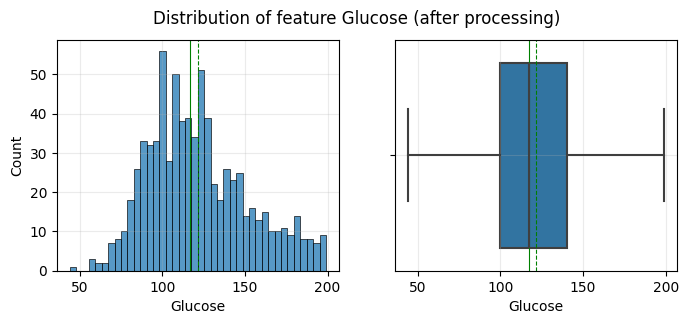
\includegraphics[width=0.7\linewidth]{images/dist - glucose - after processing.png}
    
    \vspace{-8pt}
    
    % \caption{Distribution of the feature $\mathtt{Glucose}$ (after processing)}
    
    \label{fig:dist-glucose-after}
\end{center}

% \vspace{-6pt}

Similar examinations and data cleaning procedures are conducted for other features with implausible zero values, such as $\mathtt{BloodPressure}$, $\mathtt{SkinThickness}$, $\mathtt{Insulin}$, and $\mathtt{BMI}$. Each feature is analysed for its distribution and validity, ensuring that the dataset is ready for training a classification model.


\subsection{Correlation Analysis}

\indent To visually grasp the relationships among the features, a correlation matrix is generated. Looking at the relationships between the features can help us choose the most appropriate set of features for the predictive modeling.

\vspace{-15pt}


\begin{center}
    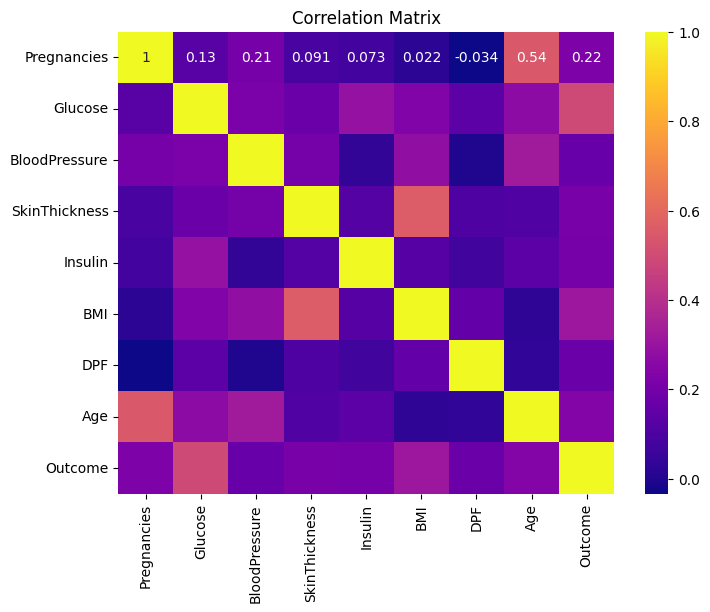
\includegraphics[width=0.8\linewidth]{images/corr - after processing - shorten.png}
    
    \caption{Correlation matrix after processing the data}
    
    \label{fig:corr-matrix-after}
\end{center}

We can see that some notable correlations exist between \texttt{SkinThickness} and \texttt{BMI}, as well as \texttt{Pregnancies} and \texttt{Age}. This suggests that each pair could be reduced to one feature to lower the dimensionality.

We can also see a significant correlation between $\mathtt{Glucose}$ and the $\mathtt{Outcome}$ variable, highlighting its potential as a significant predictor for diabetes. On the other hand, there is relatively weak correlation between $\mathtt{BloodPressure}$ and the $\mathtt{Outcome}$, suggesting its limited predictive power.

These observations can help guide the selection of features for training, which can be helpful for algorithms sensitive to high dimensionality, such as the K-Nearest Neighbours (KNN) algorithm. 
Nonetheless, in this report, all features have been utilised. 
My experimentation indicates that selecting features does not significantly improve the models' performance. 
Moreover, this allows all features in the dataset to be assessed for their relative importance.



\subsection{Target Variable Analysis}

\indent Finally, a quick look at the target variable $\mathtt{Outcome}$ reveals an imbalance in the dataset, where around 65\% of the instances indicate not having diabetes. This imbalance is 
taken into account when selecting performance metrics.



\section{Methods}

\subsection{Data Standardisation}

\indent Since our diabetes dataset is highly non-uniform, with some features having a much larger value range than others, we will apply data standardisation before passing the data to a learning model. Standardisation ensures that different features of objects are on almost the same scale, guarantees that each feature is equally important, and facilitates processing by learning algorithms.


\subsection{Choosing Models}

The following section considers a few different learning algorithms to apply to our diabetes classification problem and decides on their implementation.



\subsubsection{K-Nearest Neighbours (KNN)\cite{BenningPerra2023}}



The K-Nearest Neighbours (KNN) algorithm is one of the simplest classification methods. 
For a given input, probabilities for the class labels are computed by analysing the \( k \) nearest neighbours.
The class label corresponding to the highest probability is then chosen as the output.
In our implementation, the Euclidean distance metric is employed.
The probability is determined based on the proportion of the label. 
The label "$\mathtt{1}$" is assigned if over 50\% of the neighbours possess this label.

The number of neighbours, \( k \), is a hyperparameter that can be determined through model selection strategies. 

In this project, a grid search is conducted for \( k \) varying from 1 to 20. 
As with all classifiers, the model is evaluated using K-fold cross-validation.




\subsubsection{Logistic Regression\cite{BenningPerra2023}}


\indent Logistic regression for classification problems is similar to normal regression problems, except that the output is discrete. For binary classification, the prediction \( f(\mathbf{x}, \mathbf{w}) \) yields a probability. To achieve this, we consider \( \sigma(f(\mathbf{x}, \mathbf{w})) \) instead of \( f(\mathbf{x}, \mathbf{w}) \), where \( \sigma: (-\infty, \infty) \to [0, 1] \) is the logistic function or sigmoid function, defined as



\vspace{-12pt}

$$
\sigma(x): = \frac{1}{1+\mathrm{e}^{-x}}
$$


The goal is to solve a minimisation problem where we define and minimise a function $\mathrm{L}\left(\mathbf{w}\right): \mathbb{R}^{d+1} \to \mathbb{R}$ of $d+1$ dimensional argument $\mathbf{w}=\left(w_0,w_1,\ldots,w_{d}\right)$. Here $\mathrm{L}\left(\mathbf{w}\right)$ is called the cost function and $w_0,w_1,\ldots,w_{d}$ are the weights. 
In our model, $\mathrm{L}\left(\mathbf{w}\right)$ is linear, which simplifies finding its gradient $\nabla \mathrm{L}\left(\mathbf{w}\right)$. 
This gradient is then used in the gradient descent method to solve this minimisation problem computationally by following the update rule:


\vspace{-6pt}

$$
\mathbf{w}^{(k+1)} = \mathbf{w}^{(k)} - \tau \nabla L\left(\mathbf{w}^{(k)}\right)
$$

\vspace{-6pt}

\noindent where $\tau > 0$ is the step-size and $k\geq 0$ is the iteration number. 
In this project, $\mathbf{w}^{(0)}$ is initially set as a zero vector. % In code, I initialise $\mathbf{w}^{(0)}$ as a $d+1$ dimensional vector of zeros. 
For the K-fold cross validation demonstration, gradient descent is set to terminate when $k$ reaches $10,000$.
However, for the bootstrap sampling demonstration, 
the maximum number of iterations is reduced to 1000 to 
keep the computational runtime reasonable. % make the code more presentable. 
The hyperparameter $\tau$ is also tuned using grid search.


In this project, binary logistic regression is first implemented using only \codeword{NumPy}\cite{numpy-website} which is then compared to a \codeword{scikit-learn}\cite{sklearn-logisticregression} implementation. 
Both are trained under the same conditions using K-fold cross-validation and bootstrap sampling.


\subsubsection{Support Vector Machine (SVM)\cite{BenningPerra2023}}

\indent A limitation of logistic regression is that the hyperplane that spans the decision boundary is not necessarily optimal in the sense that it maximises the distance between the closest data points on each side of the decision boundary. 
This feature can, however, be achieved in the context of binary classification with the Support Vector Machine (SVM) algorithm. The key idea is to both maximise the distance between % $r$ of 
the closest data points to the hyper-plane and, at the same time, ensure that each data point ends up on the correct side of the decision boundary.


In this project, the \codeword{scikit-learn}\cite{sklearn_svm} library is used to implement the SVM model.



\vspace{12pt}

In addition to the three previously mentioned classification algorithms, I also experimented with a simple 2-layer neural network model. Unfortunately, the outcomes were not promising, as the model consistently predicted \( \mathtt{0} \) regardless of the input. Given that \( 65\% \) of our data are labelled \( \mathtt{0} \), this resulted in a misleading accuracy rate of about \( 65\% \), while the F1 score metric (which is described in the next section) was actually \( 0 \). Due to these limitations, I have decided not to include this model in the results section.



\section{Results and Interpretation}



This section presents the metrics and methods used to evaluate the performance of the models and interpret the results.


\subsection{Performance}

\subsubsection{F1 Score}


We have found that our dataset exhibits an imbalance, with a higher occurrence of labels marked as $\mathtt{0}$ compared to those marked as $\mathtt{1}$. 
To ensure a more reliable evaluation of the model, the F1 score\cite{F1score} is used alongside accuracy. The F1 score provides a more balanced metric, less impacted by label prevalence. Its calculation is as follows:

$$
F_1 = \frac{2 \cdot \text{precision} \cdot \text{recall}}{\text{precision} + \text{recall}}
$$

\noindent where $\text{Precision} = \frac{\text{True Positives}}{\text{True Positives} + \text{False Positives}}$ and $\text{Recall} = \frac{\text{True Positives}}{\text{True Positives} + \text{False Negatives}}$. 

\vspace{3pt}

By convention, $F_1 = 0$ when the number of true positives is 0.


\subsubsection{Performance Evaluation using K-Fold Cross Validation}

\indent To reflect the real-world performance of a model, it is important to evaluate the model using data it has not seen during training. We use K-fold cross validation to achieve this. 


Throughout this project, the number of folds $K$ is set to 5. This means that for each fold in the cross-validation process, the dataset is divided into a training set and a validation set with an $80:20$ ratio.


\subsubsection{Hyperparameter Tuning using Grid Search}


The performance of each learning algorithm depends on its hyperparameters. In the case of logistic regression, the hyperparameter is the step size \(\tau\), while for K-Nearest Neighbours (KNN), it is the number of neighbors \(k\).

A common approach to tuning these hyperparameters is to conduct a grid search. During a grid search, the model is trained multiple times using different hyperparameter values.

The results of the grid search show that, for this diabetes binary classification problem, the optimal step size for logistic regression is \(\tau = 0.01\), and the optimal number of neighbors for KNN is \(k = 11\).

For the implementations of logistic regression and Support Vector Machine (SVM) provided by \codeword{scikit-learn}\cite{sklearn-logisticregression, sklearn_svm}, the default parameters are %currently being 
used.


\subsubsection{Metrics}



Table 1 summarises the results of the experiments conducted in this project. All results were obtained using \(K\)-fold cross-validation with \(K = 5\). To ensure reproducibility, the random state was set to a consistent number \(123456789\), once before training each model. 
The results may vary to some extent depending on the randomising procedure.


The highlighted numbers in the table represent the maximum values within their respective metric categories.

    
\begin{table}[h]
\begin{center}
\begin{tabular}{|l|l|l|l|l|}
\hline
                                       & Accuracy & F1 score & Precision & Recall   \\ \hline
Logistic Regression, step size = 0.01 & 0.768254 & 0.632143 & 0.571292  & 0.710268 \\ \hline
Logistic Regression using \codeword{scikit-learn}      & 0.768254 & 0.632143 & 0.571292  & 0.710268 \\ \hline
SVM using \codeword{scikit-learn}                      & \textbf{0.773466} & \textbf{0.63687}  & 0.57163   & \textbf{0.723763} \\ \hline
KNN, k = 3                             & 0.705747 & 0.570164 & 0.55851   & 0.58545  \\ \hline
KNN, k = 11                            & 0.744835 & 0.611983 & \textbf{0.5763}    & 0.655297 \\ \hline
\end{tabular}

\caption{Average metrics of different learning algorithms}

\vspace{-12pt}

\end{center}
\end{table}



It is interesting to see that the implementation of Logistic Regression using only \texttt{NumPy}\cite{numpy-website} produced the same results as the \texttt{scikit-learn}\cite{sklearn-logisticregression} implementation, even though the optimal weight values, which will be detailed below, are different.
Assuming that the \codeword{scikit-learn} implementation is reliable and well-established, this adds confidence in the correctness of the more "primitive" implementation, although perfectly identical results may also be a cause for concern. It is also worth noting that the relatively small size of the dataset may increase the likelihood of getting the same result.


Overall, the SVM model yielded the highest results in accuracy and F1 score as well as recall, although both logistic regression implementations were also very closely matched in performance. KNN with \(k = 11\) also exhibited strong performance and achieved the highest precision, with other metrics not too far off compared to the other models. On the other hand, the worst-performing implementation was KNN with \(k = 3\), which is not surprising given that \(3\) is not the optimal hyperparameter for \(k\) in this diabetes binary classification problem.



\subsection{Feature Ranking with Bootstrap Sampling}

A natural question arises: which features hold the highest predictive power in predicting the risk of diabetes? To determine a ranking for the features, we can utilise the relative order of the optimal weights.
Instead of relying on a single set of weights,
bootstrap sampling helps us obtain a range of values for each weight which can paint a more accurate picture of the relative ordering.



In each iteration of bootstrap sampling, new samples are created by randomly selecting data points from the original dataset with replacement. In this project, these samples are of size 691 each, equivalent to %which constitutes 
90\% of the original dataset's size. 
The number of samples generated is limited to 100 to keep computational runtime manageable.
Bootstrap sampling is not applied to the K-Nearest Neighbours (KNN) model since it does not generate feature weights.



\begin{table}[h]
\begin{center}


\begin{tabular}{|l|l|l|l|}
\hline
                                                                    & \begin{tabular}[c]{@{}l@{}}Logistic Regression\\ step size = 0.01\end{tabular} & \begin{tabular}[c]{@{}l@{}}Logistic Regression \\ using \codeword{scikit-learn}\end{tabular} & SVM      \\ \hline
$\mathtt{Pregnancies}$                                                         & 0.28580                                                                        & 0.44800                                                                      & 0.34882  \\ \hline
$\mathtt{Glucose}$                                                             & \textbf{0.77665}                                                                        & \textbf{1.07446}                                                                      & \textbf{0.87862}  \\ \hline
$\mathtt{BloodPressure}$                                                       & 0.02127                                                                        & -0.09453                                                                     & -0.06719 \\ \hline
$\mathtt{SkinThickness}$                                                       & 0.09370                                                                        & 0.01352                                                                      & -0.05411 \\ \hline
$\mathtt{Insulin}$                                                             & 0.15653                                                                        & 0.18429                                                                      & 0.06856  \\ \hline
$\mathtt{BMI}$                                                                 & 0.39362                                                                        & 0.63153                                                                      & 0.47631  \\ \hline
\begin{tabular}[c]{@{}l@{}}$\mathtt{DiabetesPedigree}$\\ $\mathtt{Function}$\end{tabular} & 0.24669                                                                        & 0.28085                                                                      & 0.22302  \\ \hline
$\mathtt{Age}$                                                                 & 0.15539                                                                        & 0.12877                                                                      & 0.04258  \\ \hline
\end{tabular}

\caption{Average weights of all features after bootstrapping $100$ times}


\end{center}
\end{table}

% \vspace{-12pt}

The results are summarised in Table 2. It should be noted that these values only represent the mean weights.
We also generate some box plots for the \codeword{NumPy}\cite{numpy-website} logistic regression implementation to get a better idea of the distribution around the median. % We also use box plots to get a better idea of the distribution around the median. 
Besides slight variations in the scales of the weight values, both the logistic regression and SVM implementations within the \texttt{scikit-learn}\cite{sklearn-logisticregression, sklearn_svm} library 
produce very similar rankings of feature importance.


Based on the results obtained after employing bootstrap sampling, 
it is clear that the most important feature by far is \texttt{Glucose}, 
which makes sense given the context of predicting diabetes. \texttt{BMI} comes second in the ranking. % Following closely behind is \texttt{BMI}. 
Conversely, the features \texttt{BloodPressure} and \texttt{SkinThickness} are among the least important, as indicated by their consistently low or negligible weight values.


\begin{center}
    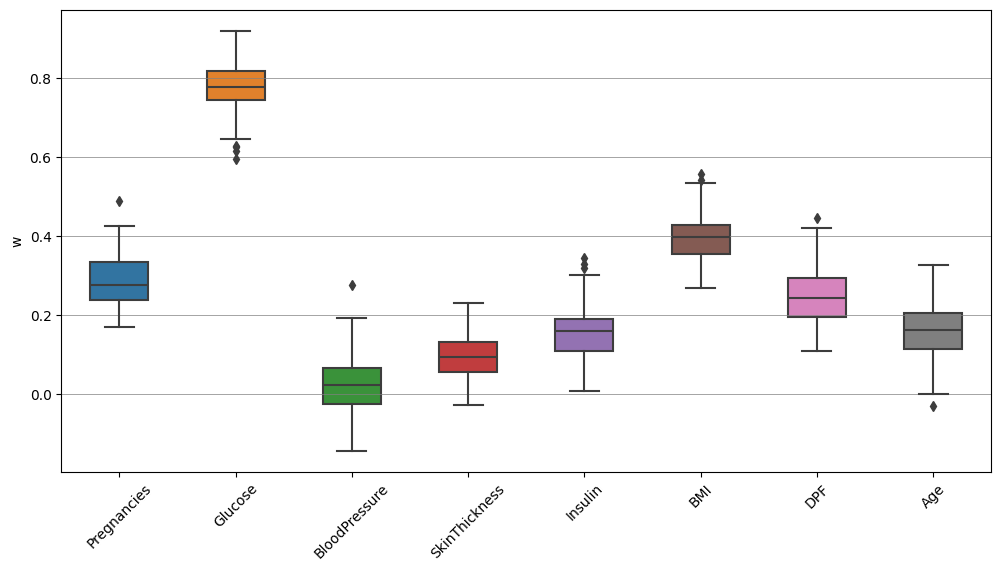
\includegraphics[width=0.8\linewidth]{images/box - weights - logistic - shorter.png}
    
    \caption{Box plots comparing the feature weights from Logistic Regression using \codeword{NumPy}}
    
    % \label{fig:box-logistic}
\end{center}

\vspace{-10pt}

% \begin{center}
%     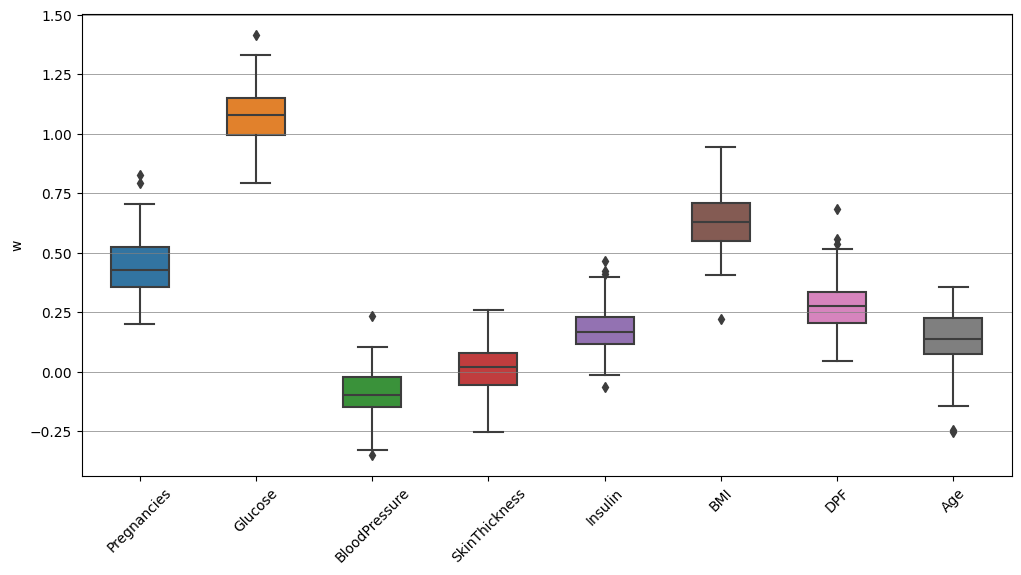
\includegraphics[width=0.6\linewidth]{images/box - weights - sklearn.png}
    
%     \caption{Box plot comparing the weights from Logistic Regression using \codeword{sklearn}}
    
%     % \label{fig:box-logistic}
% \end{center}


% \begin{center}
%     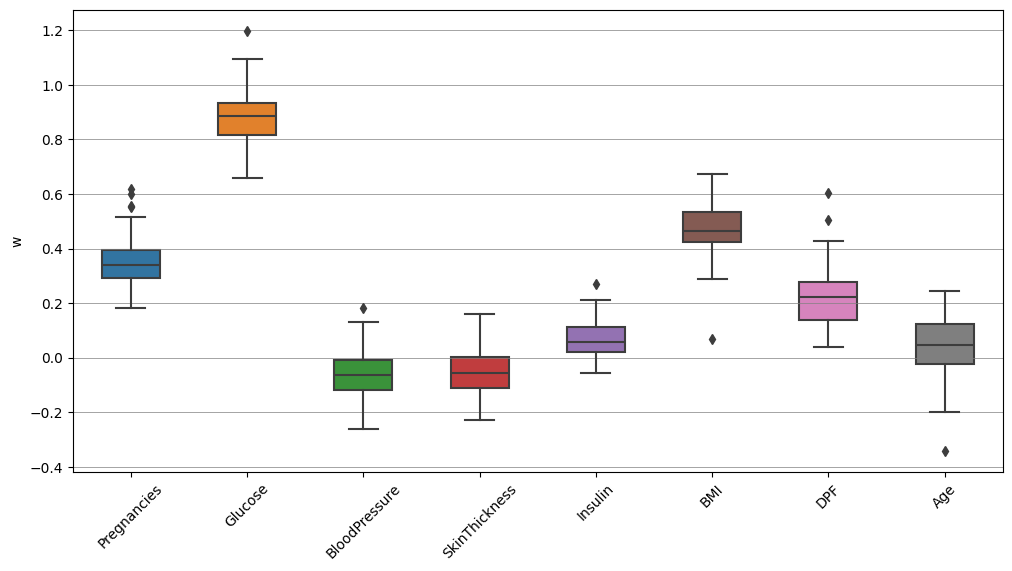
\includegraphics[width=0.6\linewidth]{images/box - weights - svm.png}
    
%     \caption{Box plot comparing the weights from SVM using \codeword{sklearn}}
    
%     % \label{fig:box-logistic}
% \end{center}






% \vspace{-12pt}

\section{Conclusion}

In this project, we examined three different learning algorithms and assessed the performance of five different implementations in solving the diabetes binary classification problem. 
The performances of these algorithms are remarkably similar when optimal hyperparameters are used.


A potential extension to % Expanding upon 
this project is the exploration of additional classification algorithms, such as decision trees and random forests. 
Additionally, within the domain of logistic regression, the introduction of regularisation parameters could be considered.

Expanding upon % Another potential extension to 
this project could also involve identifying the optimal stopping point for gradient descent. 
By plotting the result of the cost function after each iteration and observing when the curve begins to level off, we can determine the most effective number of iterations to balance accuracy and computational efficiency.

\newpage




\printbibliography


The following list contain the primary Python libraries used in the implementation of this project.

\vspace{-6pt}

\begin{itemize}
\setlength\itemsep{-0.3em}
  \item \codeword{NumPy} : for numerical representations and operations, including vector and matrix multiplication.
  \item \codeword{matplotlib} and \codeword{seaborn} : for data visualisation, including the creation of histograms and box plots.
  \item \codeword{pandas} : for data analysis and manipulation tasks, such as value replacement.
  \item \codeword{scikit-learn} : for comparisons with other learning algorithms.
  \item \codeword{random} : for generating random numbers, particularly in K-fold cross-validation and bootstrap sampling.
\end{itemize}

\end{document}